\section{Discussion}

\subsection{Fault Injection}

The fault injection campaign was intended to begin at a higher abstraction level than LLVM-IR through injecting errors in the benchmarks' source C code. These initial efforts consisted of performing an equivalent of mutation testing in the selected benchmark. This was largely misguided, as mutation testing does not make sense when it is not used to validate a test suite. 

Performing mutation testing in the tests that assert the behavior of taffo would allow discussing the developmental fault tolerance of \taffo{}, but this was hindered by the authors lack of experience with \taffo{} development and the test cases and assertions not being verbose and descriptive enough for an outsider to easily understand what the code was testing. Taking the test in listing~\ref{listing:taffo_unit_test} as an example, one can see that there is a variable annotated for use with taffo, and other variables that are not annotated. A value is returned, but there are no hints as to what the expected behavior given an input is. The function names don't help with this either, nor does the filename, which is test1.c. This makes performing mutation testing a lot more difficult. Mutation testing is used to verify that the tests actually test the behavior they describe, but when the behavior that is being tested is not described, it is all the more difficult to create mutants that target the test in question.

The README file in the simple-test-cases directory in taffo directs a potential tester to a shell script that builds and runs the test, and in the makefile the directory is marked as tests, running all the tests in the simple-test-cases directory when building taffo.

\begin{lstlisting}
    ///TAFFO_TEST_ARGS -Xvra -propagate-all


float global;

float test(float param, int notafloat)
{
  int notafloat2;
  float local __attribute((annotate("scalar(range(0, 5.0))")));
  
  local = 2.0;
  local *= param;
  local += notafloat;
  notafloat2 = local;
  return notafloat2;
}

int test2(int a)
{
  return a + 2.0;
}

\end{lstlisting}

Instead of starting with this, the initial fault injection was performed directly in LLVM-IR, through the above mentioned single bit flip experiment.

This comparison is based on injecting faults within the data that is being operated on, not on instruction bits or any other part of the program. The fault locations are selected based on operations that are only done a few of in the program, such as division, to be able to inject a fault in an equivalent location for all the different versions of the program. The comparison does not hold for anything other than an injection of faults in the data. Furthermore the fault injection has only been performed on one benchmark with a limited number of operations, therefore the results may be different in another benchmark stressing another part of the processor. 

Fixed point and floating point representations require different CPU instructions for mathematical operations. This leads to different code that uses different parts of the processor. Were a bit to be flipped in the same memory location when both programs are running, there is a high likelihood of the bit being flipped representing very different parts in the respective programs. 


The results of the fault injection campaign completed for the seidel-2d benchmark from the polybench cpu benchmark suite adapted for \taffo{} is not representative for programs compiled with \taffo{} as a whole. The changes that are made to the low-level code vary from project to project depending on the domain, and depends on what the user of the program specifies to be the range of values. 

The results from the fault injection were mostly expected: The deviations from the original answer for the floating point errors started low, then skyrocketed exponentially towards the most significant bits.




% explanation of floating point implementation
% explanation of fixed point implementatoin
% diagrams

% The LLVM-IR documentation states that when shifting the value beyond the bounds of number being shifted, you should get undefined behavior~\cite{LLVM_language_reference}. This can be seen in the experiment when attempting to inject faults in bits that don't exist. When injecting bits beyond the 64 that exist in the variable, the results become unpredictable for the fixed point implementations, and invalid for the floating point value. This however is not relevant to this thesis but concerns llvm IR behavior, and will therefore be ignored.

In the output file of the original floating point implementation without any additional faults injected, there are 19 significant digits, 16 of which is behind the decimal point. Depending on what the output is used for, an error above 1.0 could be considered to be quite a large error, or it could be insignificant. Figure~\ref{fig:graph_fixed_vs_float_error} shows a graph of the change in error when injecting an error in increasingly more significant bits in a variable. The graph cut-off is set at 1.0, this is to get a better resolution in the lower end of the fault spectrum. The deviation is the accumulated average absolute difference for each data point compared to the original floating point implementation of the program without additional faults injected. The x axis describes which bit is flipped, bit number 0 being the least significant bit.

\begin{figure}[h!]
    \centering
    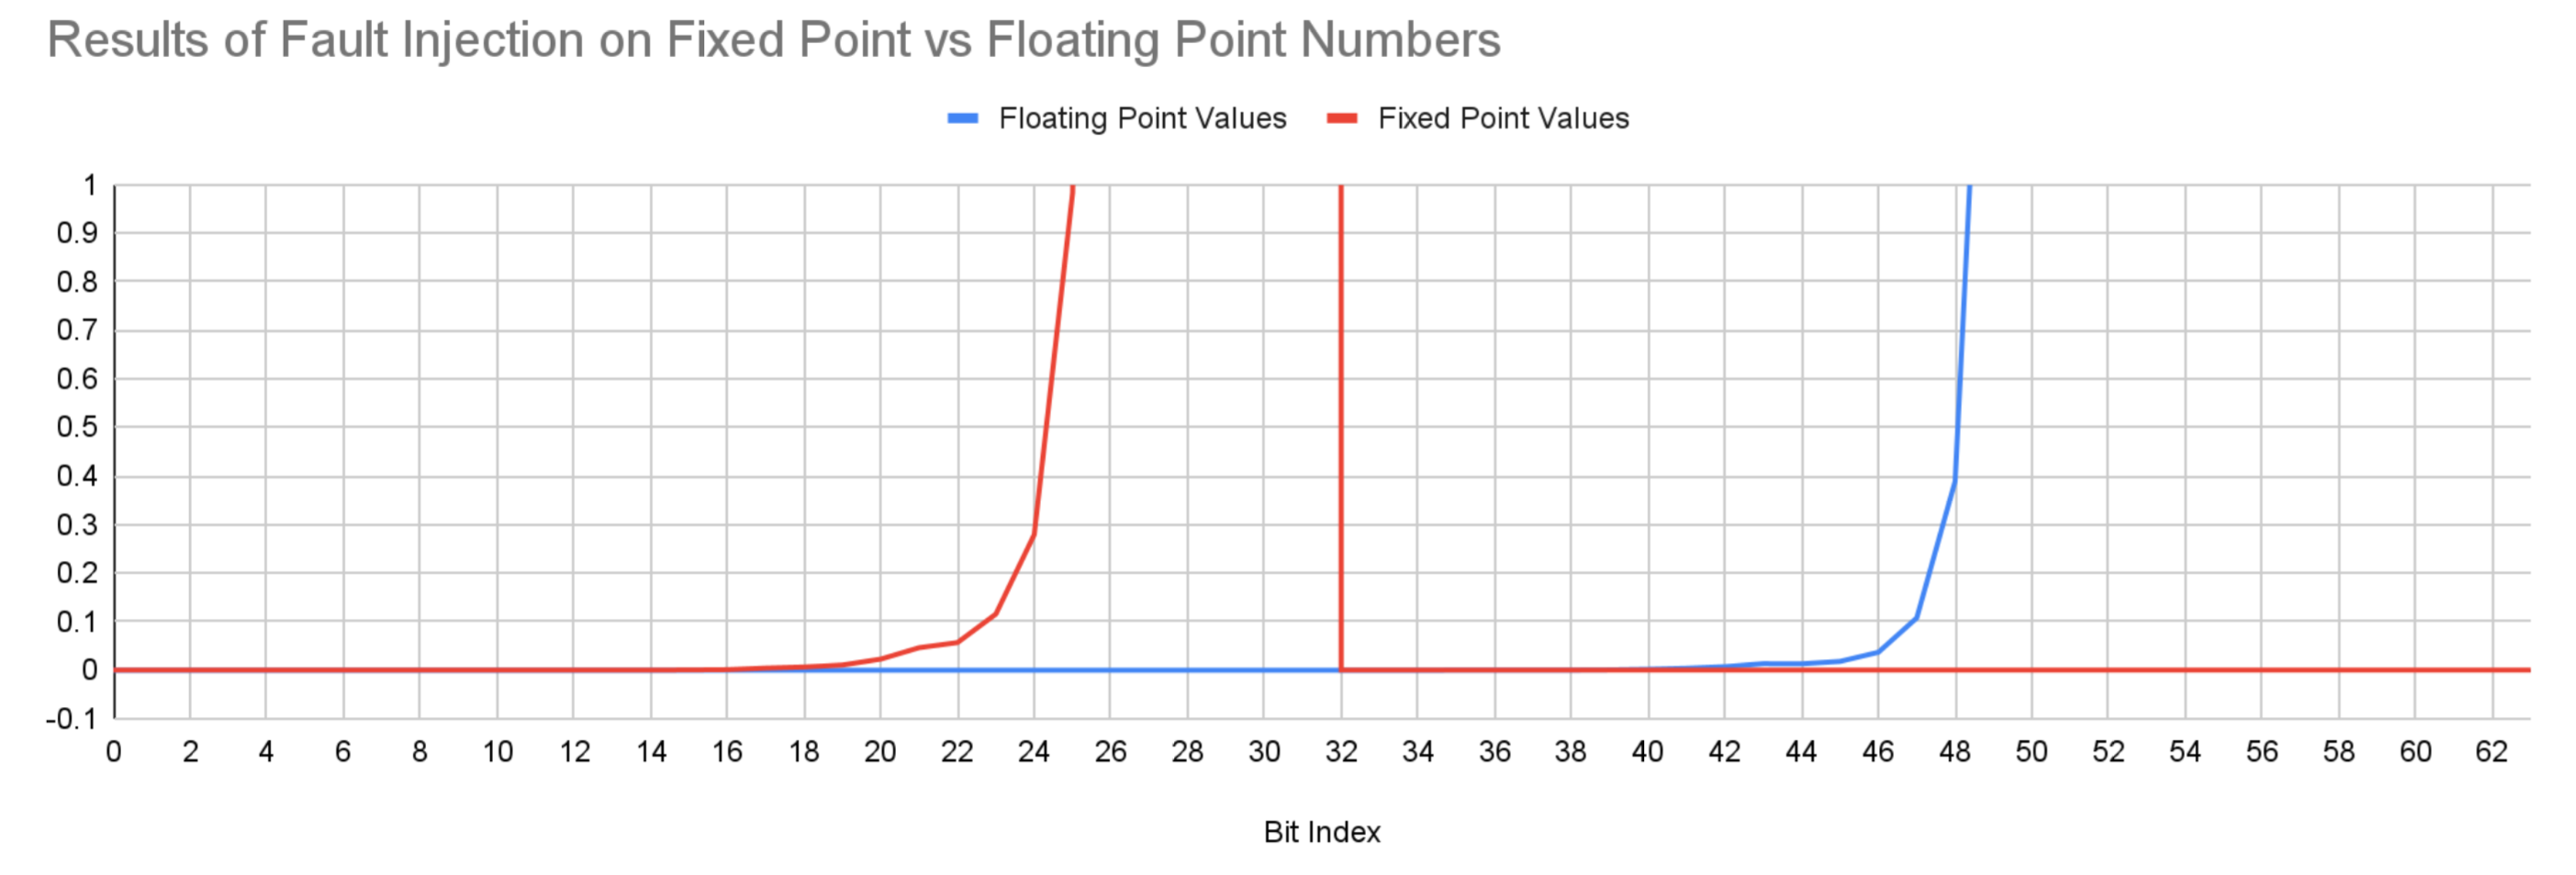
\includegraphics[width=0.5\linewidth]{Images/graph_float_vs_fixed_fault_injection_results.png}
    \caption{The graph shows how the difference from the original floating point version of the program increases the closer to the most significant bit the fault is injected. }
    \label{fig:graph_fixed_vs_float_error}
\end{figure}


The graph y axis starts at negative values even though this is not possible (the y axis is average absolute difference, therefore values will only be positive).This is to more clearly show the line for the floating and fixed point data when the error is small toward the least significant bits.

The graph shows that both the floating point values and the fixed point values seem to differ very little from the original non-fault-injected outputs. The difference in the fixed point implementation rises quickly as the injected bit approaches the the most significant bit, until suddenly dropping after injection in the bit at index 32. This can be explained by looking at the LLVM-IR that is used to inject the faults, see listing~\ref{listing:llvm_ir_fixed}. Here you can see that while the result of the division is 64 bits, from dividing two 64 bit variables, one of the operands is originally a 32 bit integer that is extended to a 64 bit number. In the final line in the listing, the result of the division and bit flip is then truncated back to a 32 bit integer, thereby discarding the injected bit if it is injected over the bit at index 31, explaining the drop in error after bit 31.

\begin{figure}[h!]
    \centering
    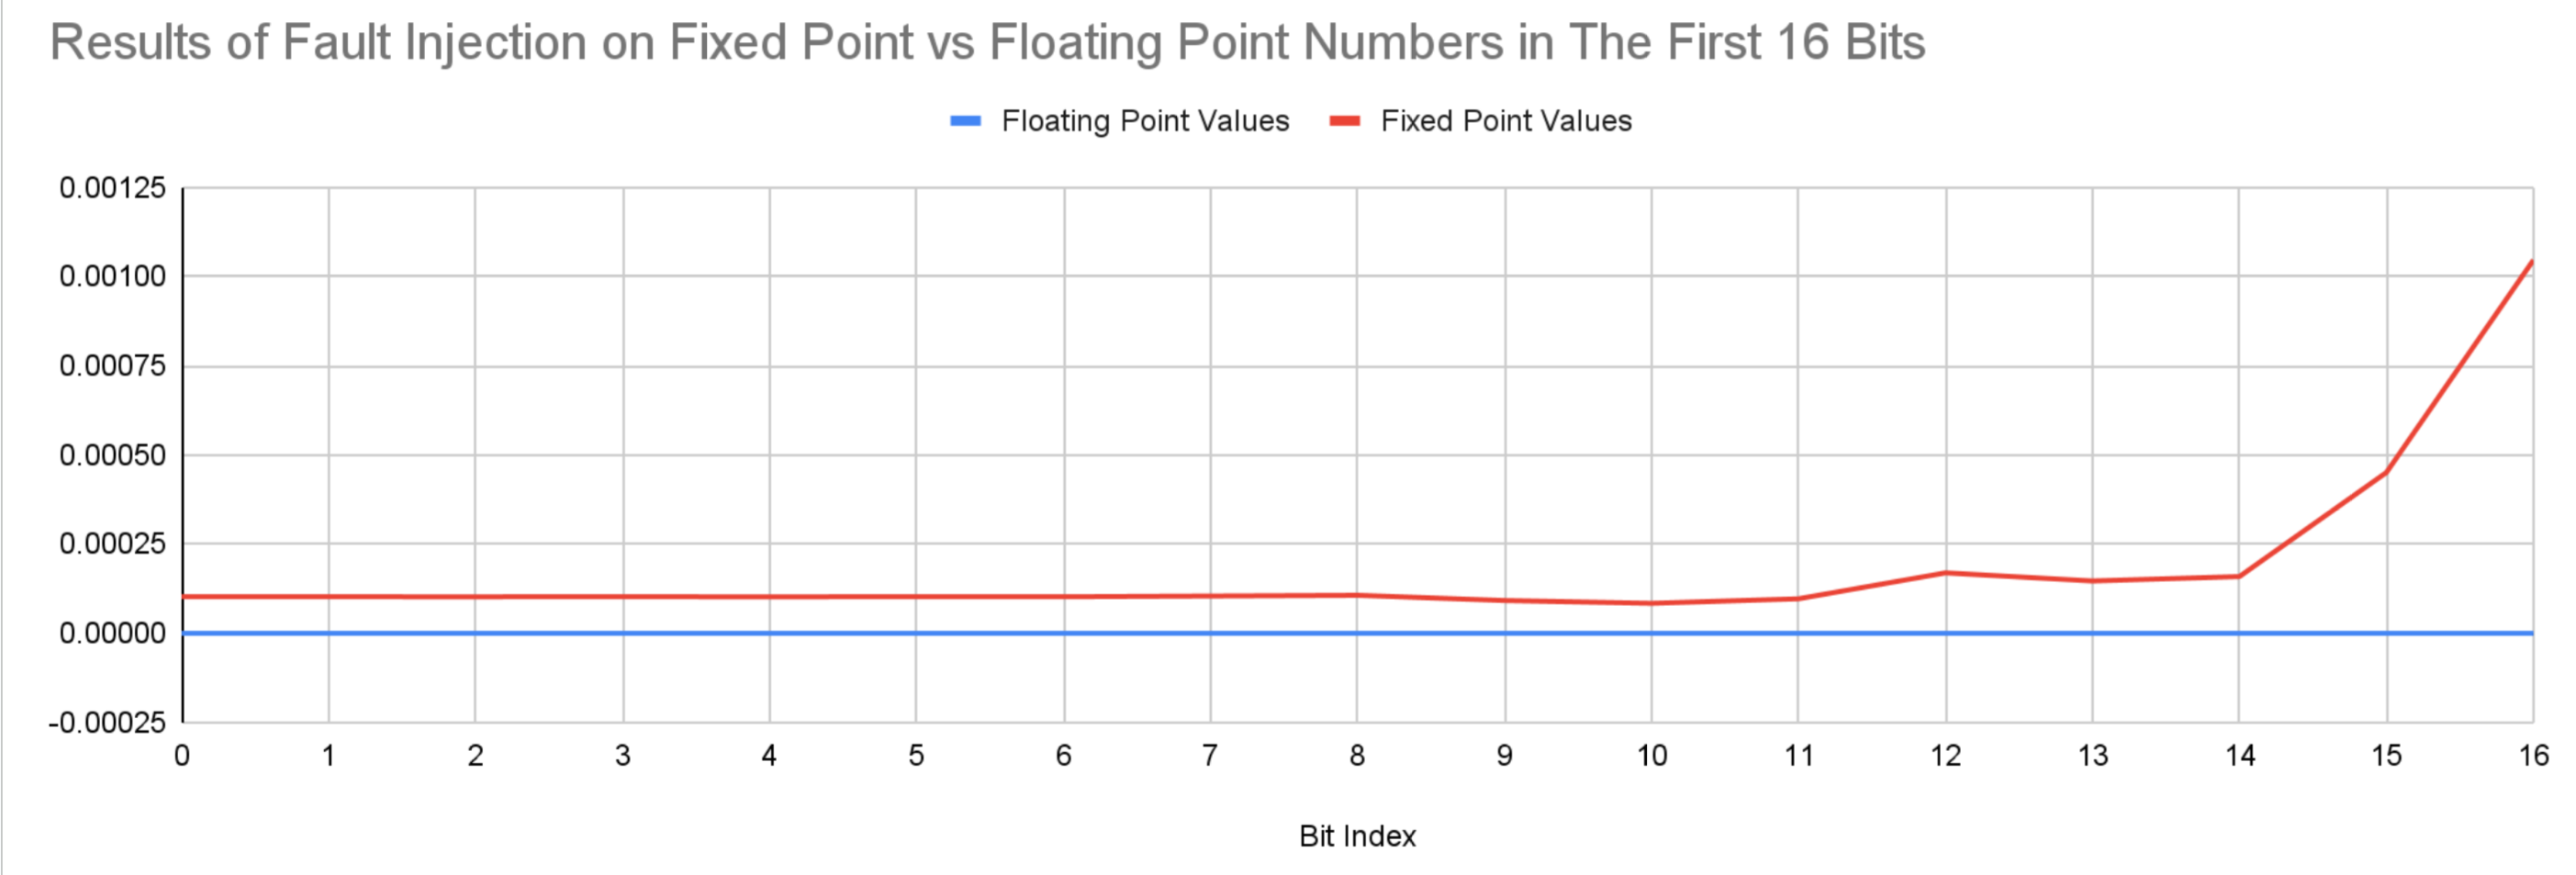
\includegraphics[width=0.5\linewidth]{graph_fault_injection_fix_vs_float_first_16_bits.png}
    \caption{The fixed point error is magnitudes larger than the floating point error at its lowest.}
    \label{fig:graph_fixed_vs_float_error_first_16}
\end{figure}

When assessing how the injected faults affect the program behavior, it is helpful to use the failure classifications found in~\citet{failure_class_with_respect_to_detection} for subtle incorrect and coarse incorrect service values. A service is the behavior of a system as percieved by an external observer. For a perfect observer, i.e. an observer that can accurately map a service output as either a correct or incorrect output. Humans are rarely perfect, which puts us in a different category of observers able to discern between three different states of service delivery: correct, coarse incorrect, and subtle incorrect.  Coarse incorrect are states that are certainly false, correct states are observably correct, and subtle incorrect states are difficult to discern as being incorrect or correct, though they are in reality the result of incorrect service. This means that a value could be percieved as correct while actually being the result of faulty service. This can counterintuitively be a bigger issue than a very large error, in that it can be more difficult to detect.

This is why the domain matters when discussing reliability. In the result, until injecting a fault in the bit at index 37, the floating point error remains lower than that of the fixed point implementation with no faults injected. In the bit at index 55, the error becomes larger than the highest error recorded for the fixed point implementations, and the error keeps rising until injecting an error at the bit in index 63, which is the sign bit.

If we define the standard fixed point version error as the threshold for a coarse error, the majority of floating point variable bit flips do not constitute a fault. 

For this benchmark, the precision was set such as to allow the use of 32 bit integers for the fixed point implementation. This was done by the authors of taffo through the use of annotations specifying the range of values that the variables can contain. This may not be the case for all the benchmarks in the included polybench benchmark suite.

% discuss the error, how error rate changes with injected bit, implications taking subtle and coarse errors into account. Subtle errors may have a larger effect on scientific calculations or highly sensitive calculations such as for satellite navigation or space travel, where if travelling very long distances a small error may result in a huge deviation. Larger errors may be easier to discover.
A larger deviation may be easier to discover than a lower deviation, either through statistics or detection algorithms. The fact that many bits in a 64-bit floating point number can be injected without a significant effect on the calculation may be an advantage if the calculation in question is fault tolerant at heart. Floating point errors go up very quickly when the error hits the exponent part of the number, so detecting a fault above a certain threshold is feasible.

On the other hand, while the smallest faults injected into fixed point numbers are larger than the smallest faults in floating point numbers, a number where only the 32 lowest bits will affect the calculations that follow have 32 bits where nothing happens when they are flipped. This is taking the huge assumption that only data bits are flipped, when this is not necessarily the case at all.




\subsection{code quality}

On a different note, the code changes of the validation script result in a more understandable piece of software.

The comparison script written for the fault injection comparison is not perfect either. However, the assumptions are documented, and tests support and explain functionality. 
%This is difficult to realize when using python as a scripting language, but at the very least variable names need to be descriptive, and file outputs need to follow the existing standards and descriptions (for instance not mislabeling an output as a .csv file).

Some changes were apparent not because of the programming skills of the author, but simply because of an IDE tool highlighting errors that were easy to remedy. Figure~\ref{fig:IDE_highlighting} shows the highlighted error, which in this case is a keyword that does nothing. In this case the error is that the code describes functionality that is not possible.

\begin{figure}[h]
    \centering
    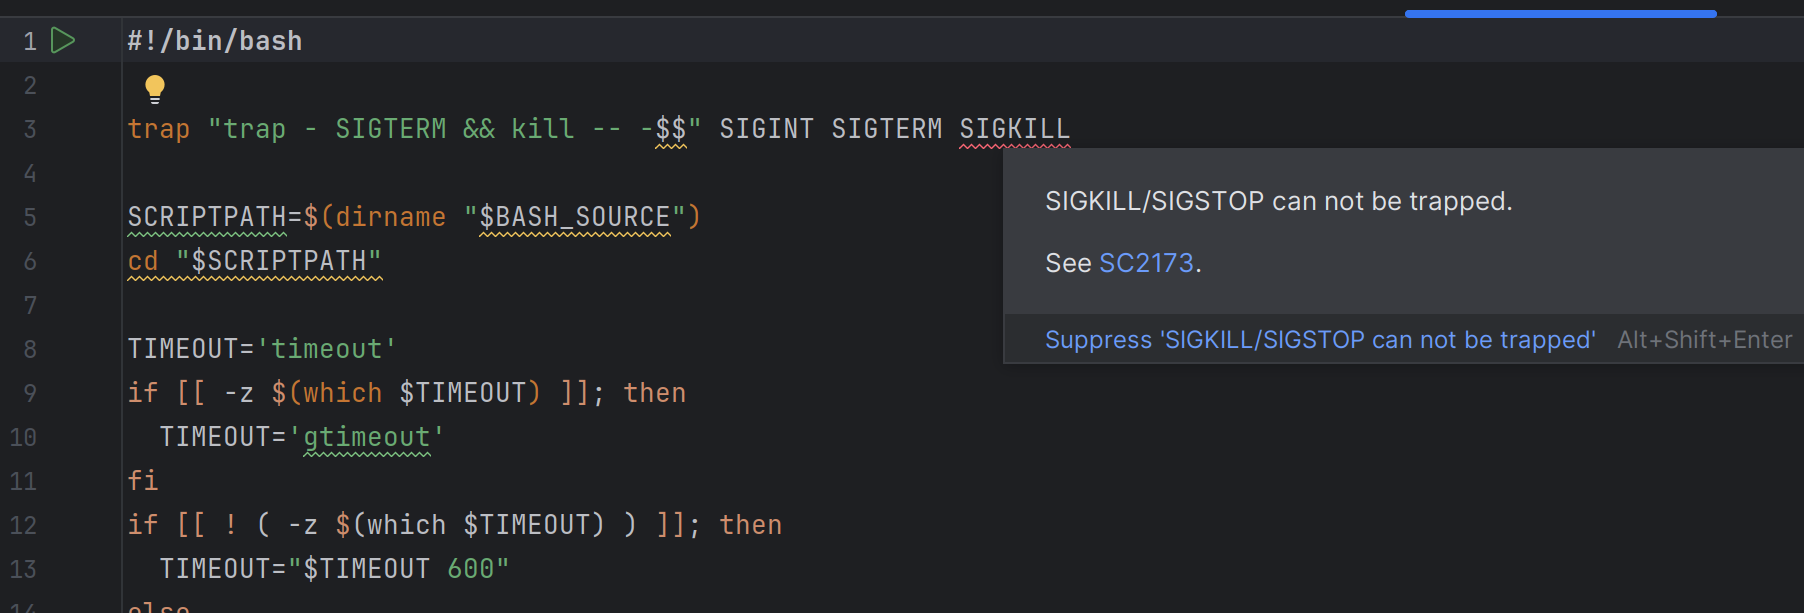
\includegraphics[width=0.5\linewidth]{Images/IDE_highlighting.png}
    \caption{the IDE, in this case CLion, highlighting an error in a shell script.}
    \label{fig:IDE_highlighting}
\end{figure}
% There is a habit of writing code as if to be archived forever. The documentation lags behind, and there is no test suite for the tool

There are many aspects of programming that can be measured to provide an indication of code quality. One such example is test coverage, which measures how many lines of the written code is executed through tests, and a higher percentage of code executed in tests is better. Although a program has 100\% code coverage, this alone does not designate the program as a good program: The tests themselves need to specify what behavior they test, and the test needs to assert that the output aligns with the expected output, such that if there is a change in the code that changes this behavior the test should fail. Quantitative code quality metrics are intended to be used as an aid in writing good code, not as designators of good or bad code. 

Using quantitative code quality metrics is a more reliable qualifier of bad code. Taking coverage again as the example metric, while a high coverage cannot be used alone to decide whether code is well written or not, a low coverage is a good indication of code that doesn't follow standard development practices.  


\subsection{Differences between documentation and implementation}

There have been some omissions and deviations which are not documented in neither the code repository nor the papers which can be submitted as a pull request to the \taffo{} project. 
This includes facts such as the error propagator not actually doing anything, and the installation instructions of \taffo{} not being foolproof, at least not for the fool of a thesis author.

Though there is both a test and a test-lit folder in the \taffo{} project neither is documented in the readme or elsewhere, and the tests themselves are cryptic at best. This last fact may be due to the design of lit itself, which requires some knowledge of the framework to understand the tests. 

In addition to not being very declarative in the test descriptions, the tests folder contains a lot of benchmarks. These are not tests in that they do not assert some kind of functionality that can be verified, only whether the code produces \*some\* output. Therefore it should not reside in the tests folder, but perhaps a folder named benchmarks.

\taffo{}, when called using the parameters in the existing compile script, produces llvm ir files. These files are numbered according to which step they represent in the taffo compilation process. \taffo{} has a flag called emit-llvm that is supposed to emit LLVM-IR, and does so, but this llvm-ir file is not linked to neccessary files, and does not run. This is confusing. 
To get llvm ir that is linked you need to either link it manually, or take the existing LLVM-IR intermediate files. this was discovered through troubleshooting. 
